%!TEX root = ../main.tex

We implemented the algorithm in Section~\ref{sec:algorithm} on top of OSTRICH, resulted to a string solver called $\ostrichrecl$. 
%
In this section, we evaluate the performance of $\ostrichrecl$ on two benchmark suites, that is, RegCoL and AutomatArk. In the sequel, we first describe the two benchmark suites as well as the experiment setup. Then we present the experiment results. 
We do experiments to compare the performance of $\ostrichrecl$ with the state-of-the-art string solvers. Moreover, in order to know whether $\ostrichrecl$ is good at solving string constraints with large counting and length bounds, we extract 1,969 instances with large bounds out of the two benchmark suites, and compare the performance of $\ostrichrecl$ with the other solvers on these instances. Finally, we empirically justify the technical choices made in the decision procedure of Section~\ref{subsec:cefadec} by comparing $\ostrichrecl$ with the following two variants of $\ostrichrecl$: $\ostrichrecl_{\rm - ASR}$ and $\ostrichrecl_{\rm NUXMV}$, where $\ostrichrecl_{\rm - ASR}$ and $\ostrichrecl_{\rm NUXMV}$ are obtained from $\ostrichrecl$ by removing the automata size-reduction technique (i.e. Step 2 in Section~\ref{subsec:cefadec}) and using the nuXmv model checker to solve the nonemptiness of $\cefadec$ respectively. 
 
%including the results for an overall evaluation as well as the results on the benchmark instances with large bounds. Moreover, we do experiments to show the effectiveness of the automata size-reduction technique (i.e. Step 2 in Section~\ref{sec:algorithm}) as well as compare $\ostrichrecl$ with the  nuXmv-based approach in \cite{atva2020}.  

%Then we present experiment results of the large-counting part and evaluate the simplification techniques. The goal of our experiments is to answer the following questions:
%\begin{itemize}
%  \item [Q1:] Does the decision procedure perform well~(Sec \ref{subsec:overall_eval}), especially when the counting bounds are large?~(Sec \ref{subsec:large_bounds_eval})
%  \item [Q2:] Are the size-reduction techniques practical?~(Sec \ref{subsec:size_reduction_eval})
%  \item [Q3:] How effective is the algorithm for solving the nonemptiness problem compared to the case that uses the nuXmv model checker~\cite{atva2020}?~(Sec \ref{subsec:size_reduction_eval})
%\end{itemize}



\subsection{Benchmark suites and experiment setup}\label{sec:bench}

Our experiments utilize two benchmark suites, namely, \emph{RegCoL} and \emph{AutomatArk}. Other industrial benchmark suites are not utilized because they contain no counting operators. There are 48,843 instances in total, and all benchmark instances are in the SMTLIB2 format.
Moreover, it turns out that only 5\% of regexes among the 48,843 instances are non-register-representable (see Section~\ref{subsec:regex2cefa}).

\medskip
\noindent
\emph{RegCoL benchmark suite.} There are 40,628 RECL instances in the RegCoL suite. These instances are generated by extracting regexes with counting operators from the open source regex library \cite{regex_lingua_franca,redos_lenka} and manually constructing a RECL constraint $x \in e \wedge x \in e_{sani} \wedge |x| > 10$ for each regex $e$,
where $e_{sani} \equiv \overline{\Sigma^*(<+ >+'+''+\&)\Sigma^*}$ is a regular expression that sanitizes all occurrence of special characters $<$, $>$, $'$, $''$, or $\&$. 
The expression $e_{sani}$ is introduced in view of the fact that these characters are usually sanitized in Web browsers to alleviate the XSS attacks \cite{malware_detection_3_kudzu,CCH_18}.

\medskip
\noindent
\emph{AutomatArk benchmark suite.}
This benchmark suite is adapted from the AutomatArk suite \cite{z3str3re} by picking out the string constraints containing counting operators. We also add the length constraint $|x| > 10$ for each string variable $x$. There are 8,215 instances in the AutomatArk suite.
Note that the original AutomatArk benchmark suite \cite{z3str3re} includes 19,979 instances, which are conjunctions of regular membership queries generated out of regular expressions in \cite{automatark}.

\medskip
\noindent
\emph{Distribution of problem instances w.r.t. counting bounds. }
The distribution of problem instances w.r.t. the counting bounds in RegCoL and AutomatArk suites is shown in Fig~\ref{fig:count_distri}, where the $x$-axis represents the counting bound and the $y$-axis represents the number of problem instances whose maximum counting bound is equal to the value of the $x$-axis. 
%The upper bound is the number $n$ of regex $e^{\{m,n\}}, e^{\{n,n\}}$ and $e^{\{n,\infty\}}$ (which is equivalent to $e^{\{n,n\}}e^*$). 
From Fig~\ref{fig:count_distri}, we can see that while most problem instances contain only small bounds, there are still around 2,000  (about 4\%) of them using large counting bounds (i.e. greater than or equal to $50$).
%Although most upper bounds are small, about two thousand of them are still greater than 50. 

\medskip
\noindent
\emph{Experiment setup.}
All experiments are conducted on CentOS Stream release 8 with 4 Intel(R) Xeon(R) Platinum 8269CY 3.10GHz CPU cores and 190 GB memory. We use the \textsc{zaligvinder} framework \cite{zaligvinder_2021} to execute the experiments, with a timeout of 60s for each instance.


%
\begin{figure}[ht]
\vspace{-2mm}
  \centering
  \begin{subfigure}[t]{0.49\textwidth}
    \centering\vskip 0pt
    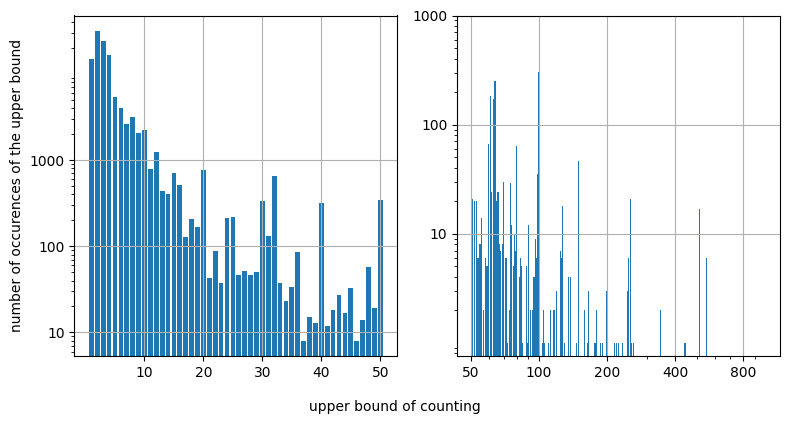
\includegraphics[width=0.9\textwidth]{counting_distribution.png}  
    \caption{Distribution of problem instances w.r.t. counting bounds}  
    \label{fig:count_distri}
  \end{subfigure}
  \hfill
  \begin{subfigure}[t]{0.49\textwidth}
    \centering\vskip 0pt
      \import{tables}{table_regcol.tex}
      \caption{Overall performance evaluation}
    \label{fig:table_overall_eval}
  \end{subfigure}
  \caption{Distribution of counting bounds and performance evaluation}
\vspace{-7mm}
\end{figure}

\subsection{Performance evaluation}\label{subsec:overall_eval}

We evaluate the performance of $\ostrichrecl$ against the state-of-the-art string constraint solvers, including CVC5
\cite{cvc5}, Z3seq \cite{z3seq}, Z3str3
\cite{Z3-str3}, Z3str3RE \cite{BD+23}, and OSTRICH
\cite{CHL+19}, on RegCoL and AutomatArk benchmark suites.
The experiment results can be found in Figure~\ref{fig:table_overall_eval}. Note that we take the results of CVC5 as the ground truth\footnote{Initially,  we used the majority vote of the results of the solvers as the ground truth. Nevertheless, on some problem instances, all the results of the three solvers in the Z3 family are wrong (after manual inspection), thus failing this approach on these instances.}, and the results different from the ground truth are classified as \emph{soundness error}. We can see that $\ostrichrecl$ solves almost all 48,843 instances, except 182 of them, that is, it solves 48,662 instances correctly. The number is 3,908/1,111/12,838/2,306/2,396 more than the number of instances solved by CVC5/Z3str3RE/Z3str3/Z3seq/OSTRICH respectively.
%
Moreover, $\ostrichrecl$ is the second fastest solver, whose average time on each instance is close to the fastest solver Z3str3RE (1.93s versus 1.62s). 

%To answer \textbf{Q1}, \textbf{$\ostrichrecl$ is the second fastest solver on these benchmark suites, and it solves the most number of instances}.

%


\subsection{Evaluation on problem instances with large bounds}\label{subsec:large_bounds_eval}

We extract 1,969 problem instances with large counting bounds (greater than or equal to $50$) from the RegCoL and AutomatArk benchmark suites.  
Moreover, in order to test the performance of the solvers on string constraints with large length bounds as well, we increase the length bound to $200$, that is, $|x| > 200$.

We evaluate the performance of $\ostrichrecl$ on the 1,969 instances. 
The experiment results can be found in Table~\ref{tab:large-bound}. We can see that $\ostrichrecl$ solves 1,873 instances correctly, which is 947/278/563/637/523 more than those solved by CVC5/Z3str3RE/Z3str3/Z3seq/OSTRICH respectively. Furthermore, $\ostrichrecl$ is 6.79/2.88/2.61/5.27/3.95 times faster than CVC5/Z3str3RE/ Z3str3/Z3seq/OSTRICH respectively. From the results, we can conclude that $\ostrichrecl$ is much more effective and efficient to solve the problem instances with large bounds than the other solvers.  
%To answer \textbf{Q1}, we can see that $\ostrichrecl$ \textbf{is far more efficient than the other solvers on problem instances with large bounds.}

\begin{table}
\vspace{-2mm}
  \centering
  \begin{subtable}{0.53\textwidth}
      \centering
    \import{tables}{table_large_count.tex}
      \caption{Large bounds}
      \label{tab:large-bound}
  \end{subtable}
  \begin{subtable}{0.45\textwidth}
      \centering
      \import{tables}{table_simp.tex}
      \caption{Empirical justification of the technical choices in the decision procedure}
      \label{tab:results_simp}
  \end{subtable}
  \caption{More experiment results, where the time limit is set as 60 seconds}
\vspace{-8mm}
\end{table}


\subsection{Empirical justification of the technical choices made in the decision procedure}\label{subsec:size_reduction_eval}
%
%We also do experiments to evaluate the effectiveness of the automata size-reduction techniques, that is, Step 2 in Section~\ref{subsec:cefadec}. 
%Let us use $\ostrichrecl_{\rm -SIMP}$ to denote $\ostrichrecl$ with the size-reduction techniques removed. 
We compare $\ostrichrecl$ with $\ostrichrecl_{\rm -ASR}$ and $\ostrichrecl_{\rm NUXMV}$, to justify the technical choices made in Section~\ref{subsec:cefadec}. 
The experiment results can be found in Table~\ref{tab:results_simp}. 
We can see that $\ostrichrecl$ solves 1,503 more instances and is 2.21 times faster than $\ostrichrecl_{\rm -ASR}$. Therefore, the automata size-reduction technique indeed plays an essential role in the performance improvement. 
%To answer \textbf{Q2}, \textbf{the size-reduction techniques indeed play a vital role in the performance improvement}. 
Moreover, $\ostrichrecl$ solves 1,798 more instances and is 3.13 times faster than $\ostrichrecl_{\rm NUXMV}$. Therefore, the decision procedure in Section~\ref{subsec:cefadec} is more efficient to solve the $\cefadec$ problem than nuXmv. 

%To answer \textbf{Q3}, \textbf{our algorithm for solving the nonemptiness problem is much better than the \textsc{nuXmv}-based techniques}.
